\section{Zielsetzung}
In diesem Versuch werden gedämpfte und erzwungene Schwingungen untersucht.
Dazu wird der Dämpfungswiderstand der gedämpften Schwingung ermittelt,
sowie Resonanzphänomene der erzwungenen Schwingung betrachtet.

\section{Theoretische Grundlage}

\subsection{Gedämpfte Schwingung}
\noindent
In einem Stromkreis der aus einer Kapazität C und einer Induktivität L besteht, 
schwingt die Energie zwischen diesen beiden Speicherelementen ungedämpft hin und her.
Wird der Schaltung ein ohmscher Widerstand R hinzugefügt,
kommt es zu einer Dämpfung, 
da die elektrische Energie irreversibel in Joulsche Wärme umgewandelt wird.
Der Aufbau dieser Schaltung ist in Abbildung (\ref{fig:gedaempft}) dargestellt.

\begin{figure}
    \centering
       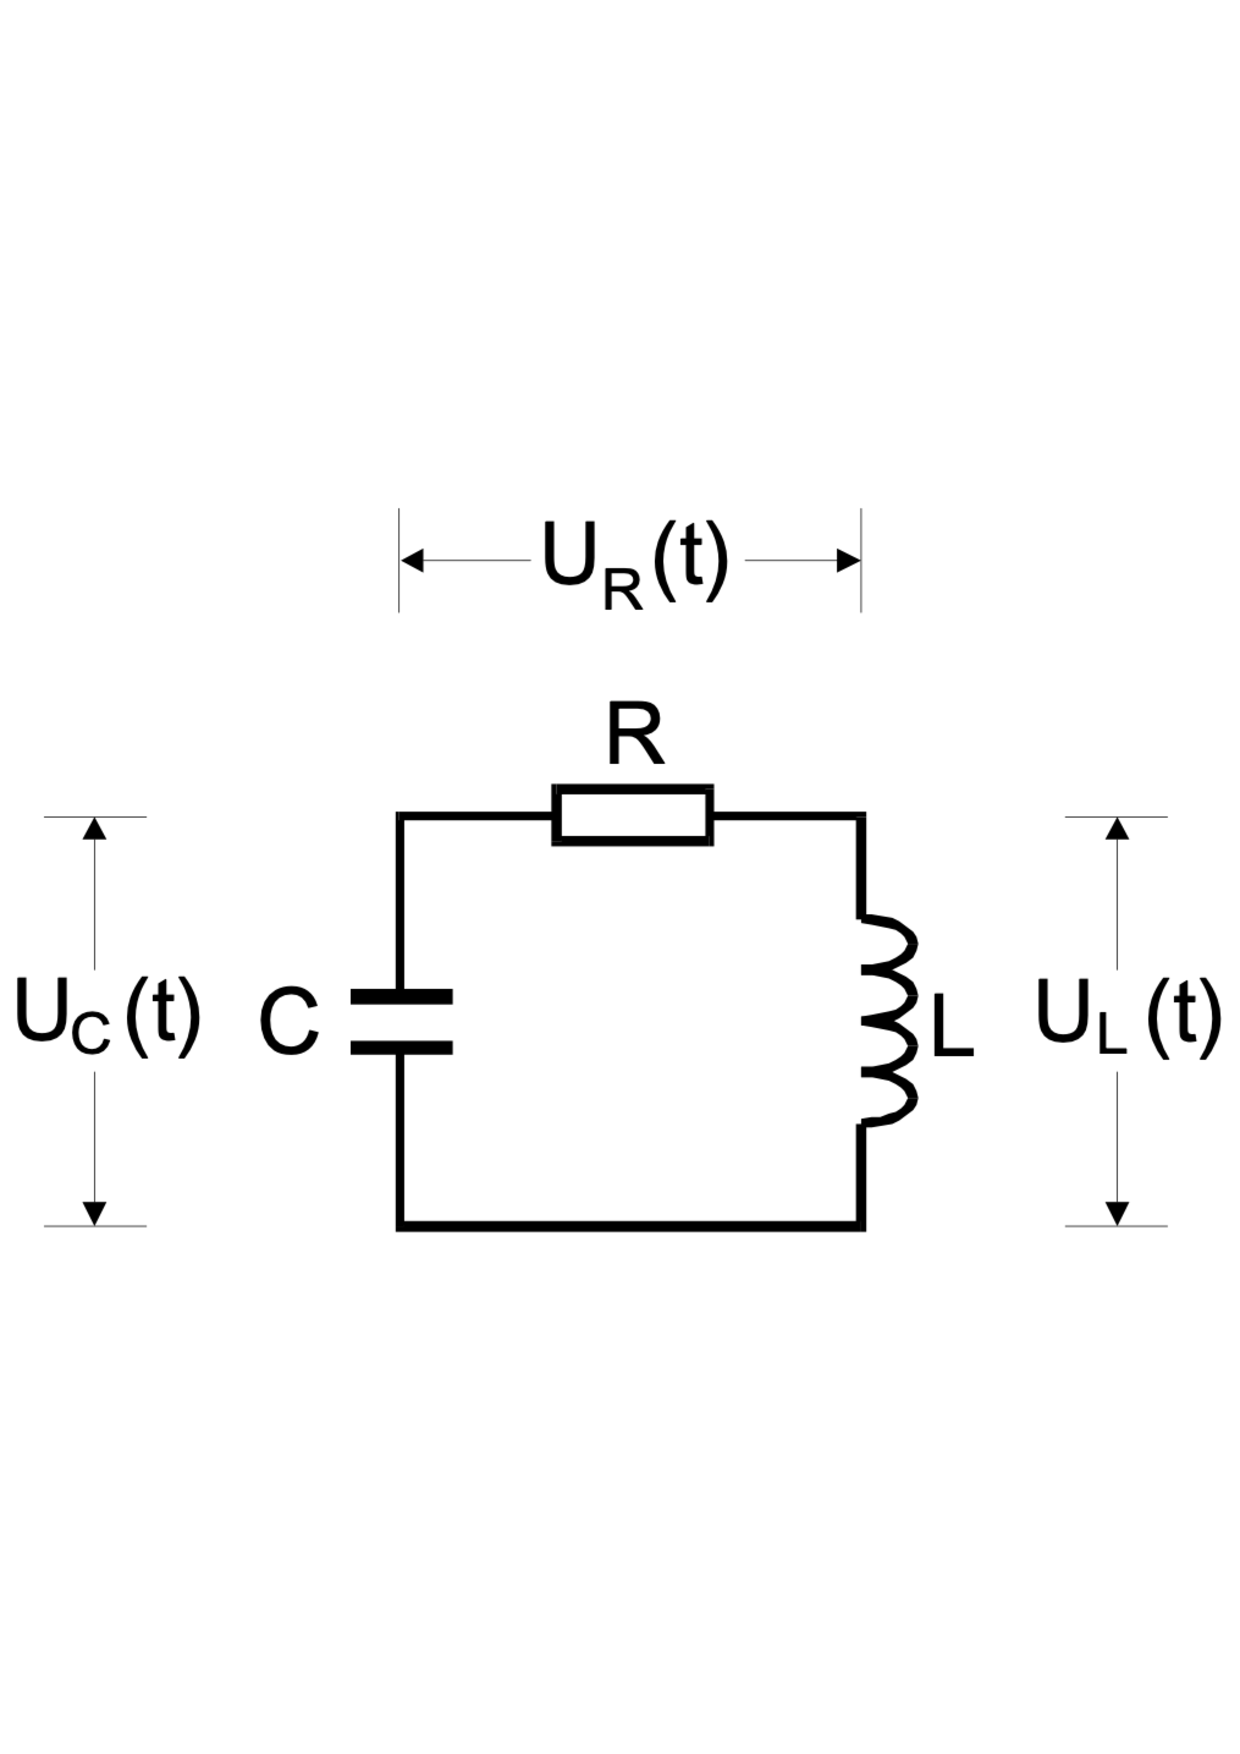
\includegraphics[height=5cm]{gedaempft.pdf}
       \caption{Schaltplan zur Erzeugung einer gedämpften Schwingung (Quelle: \cite{V354}).}
       \label{fig:gedaempft}
\end{figure}

\noindent
Mithilfe des 2. Kirchhoff'schen Gesetzes und einfachen Umformungen kann eine Differentialgleichung für den Strom I(t) der gedämpften Schwingung aufgestellt werden.
Sie hat die Gestalt:

\begin{equation}
\frac{\text{d}^2 I}{\text{dt}^2} + \frac{R}{L} \frac{\text{d} I}{\text{dt}} + \frac{1}{LC}I = 0.
\label{eqn:dgl}
\end{equation}

\noindent
Mit geeignetem Ansatz lässt sich die Differentialgleichung lösen 
und für die konstante Frequenz $\omega$ ergibt sich:

\begin{equation}
\omega_{1,2} = j \frac{R}{2L} \pm \sqrt{\frac{1}{LC} - \frac{R^2}{4L^2}} .
\end{equation}

\noindent
Abhängig von dem Term unter der Wurzel wird im Folgenden zwischen 2 Fällen unterschieden.

\newpage
\begin{enumerate}
    \item Fall: \textbf{Schwingfall} $\frac{1}{LC} > \frac{R^2}{4L^2}$

    Beim Schwingfall ergibt sich eine reeller Wurzelterm und es entsteht eine harmonische Schwingung,
deren Amplitude mit zunehmender Zeit gegen Null geht.
Ihr Verlauf ist in Abbildung (\ref{fig:schwingfall}) dargestellt.

\begin{figure}
    \centering
       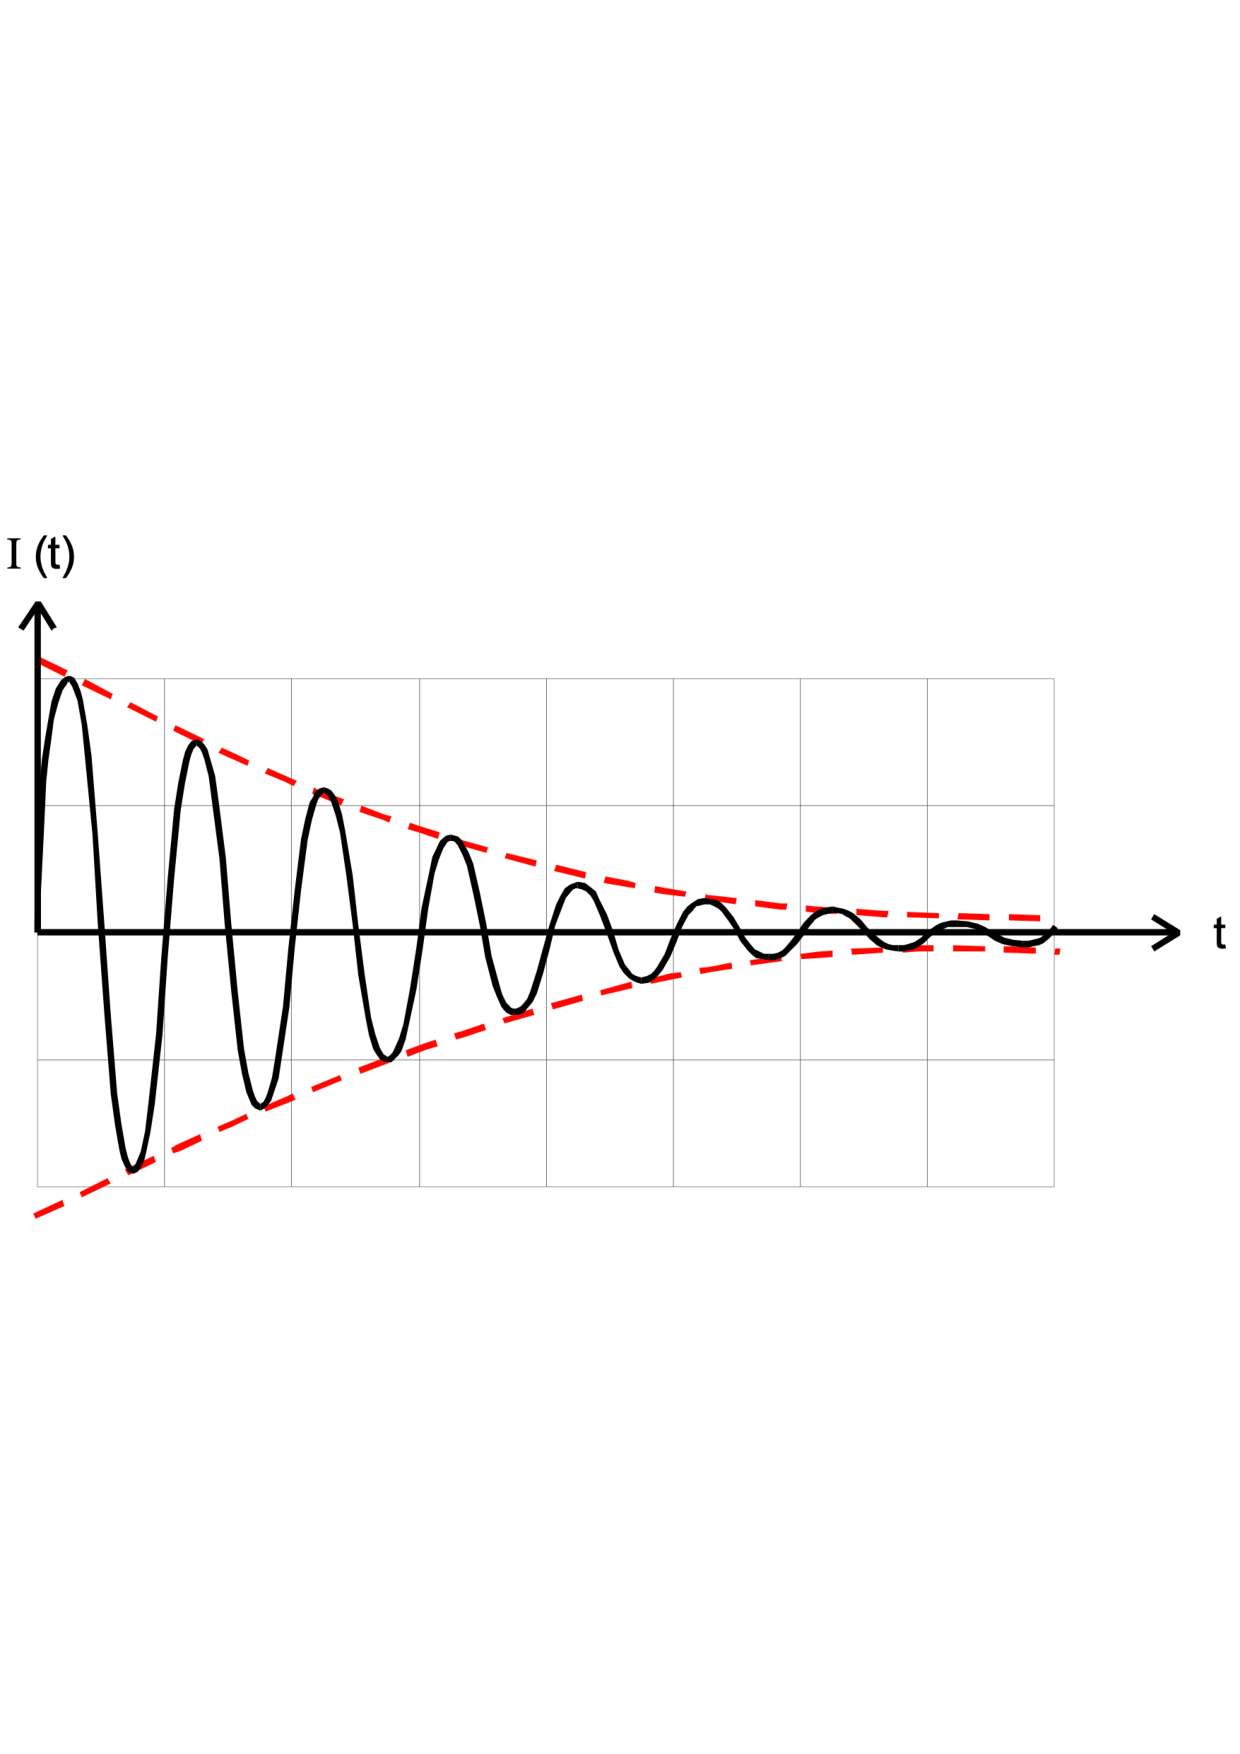
\includegraphics[height=5cm]{schwingfall.pdf}
       \caption{Schwingfall eines RCL-Kreises (Quelle: \cite{V354}).}
       \label{fig:schwingfall}
\end{figure}

Die Einhüllende ist eine e-Funktion der Form 

\begin{equation}
\pm U_0 e^{-2\pi\mu t}
\label{eqn:einh}
\end{equation}

und die Abklingdauer, die Zeit nach der die Amplitude auf den e-ten Teil ihres ursprünglichen Wertes reduziert wurde,
lässt sich schreiben als:

\begin{equation}
T_{ex} = \frac{1}{2\pi\mu} = \frac{2L}{R}.
\end{equation}

\item Fall: \textbf{Aperiodischer Grenzfall} $\frac{1}{LC} < \frac{R^2}{4L^2}$

In diesem Fall ist der Wurzelterm eine imaginäre Zahl und die Lösung für I(t) enthält keinen oszillatorischen Anteil mehr.
In diesem Versuch soll nur der Spezialfall $\frac{1}{LC} = \frac{R^2}{4L^2}$ betrachtet werden, 
bei der die Stromstärke I(t) ohne Überschwingen am schnellsten gegen Null geht, 
wie es die gestrichelte Linie in Abbildung (\ref{fig:grenzfall}) darstellt.
Der Widerstand, der den aperiodischen Grenzfall hervorruft ist definiert als:

\begin{equation}
    R_{ap} = 2\sqrt{\frac{L}{C}}
\label{eqn:rap}
\end{equation}

\begin{figure}
    \centering
       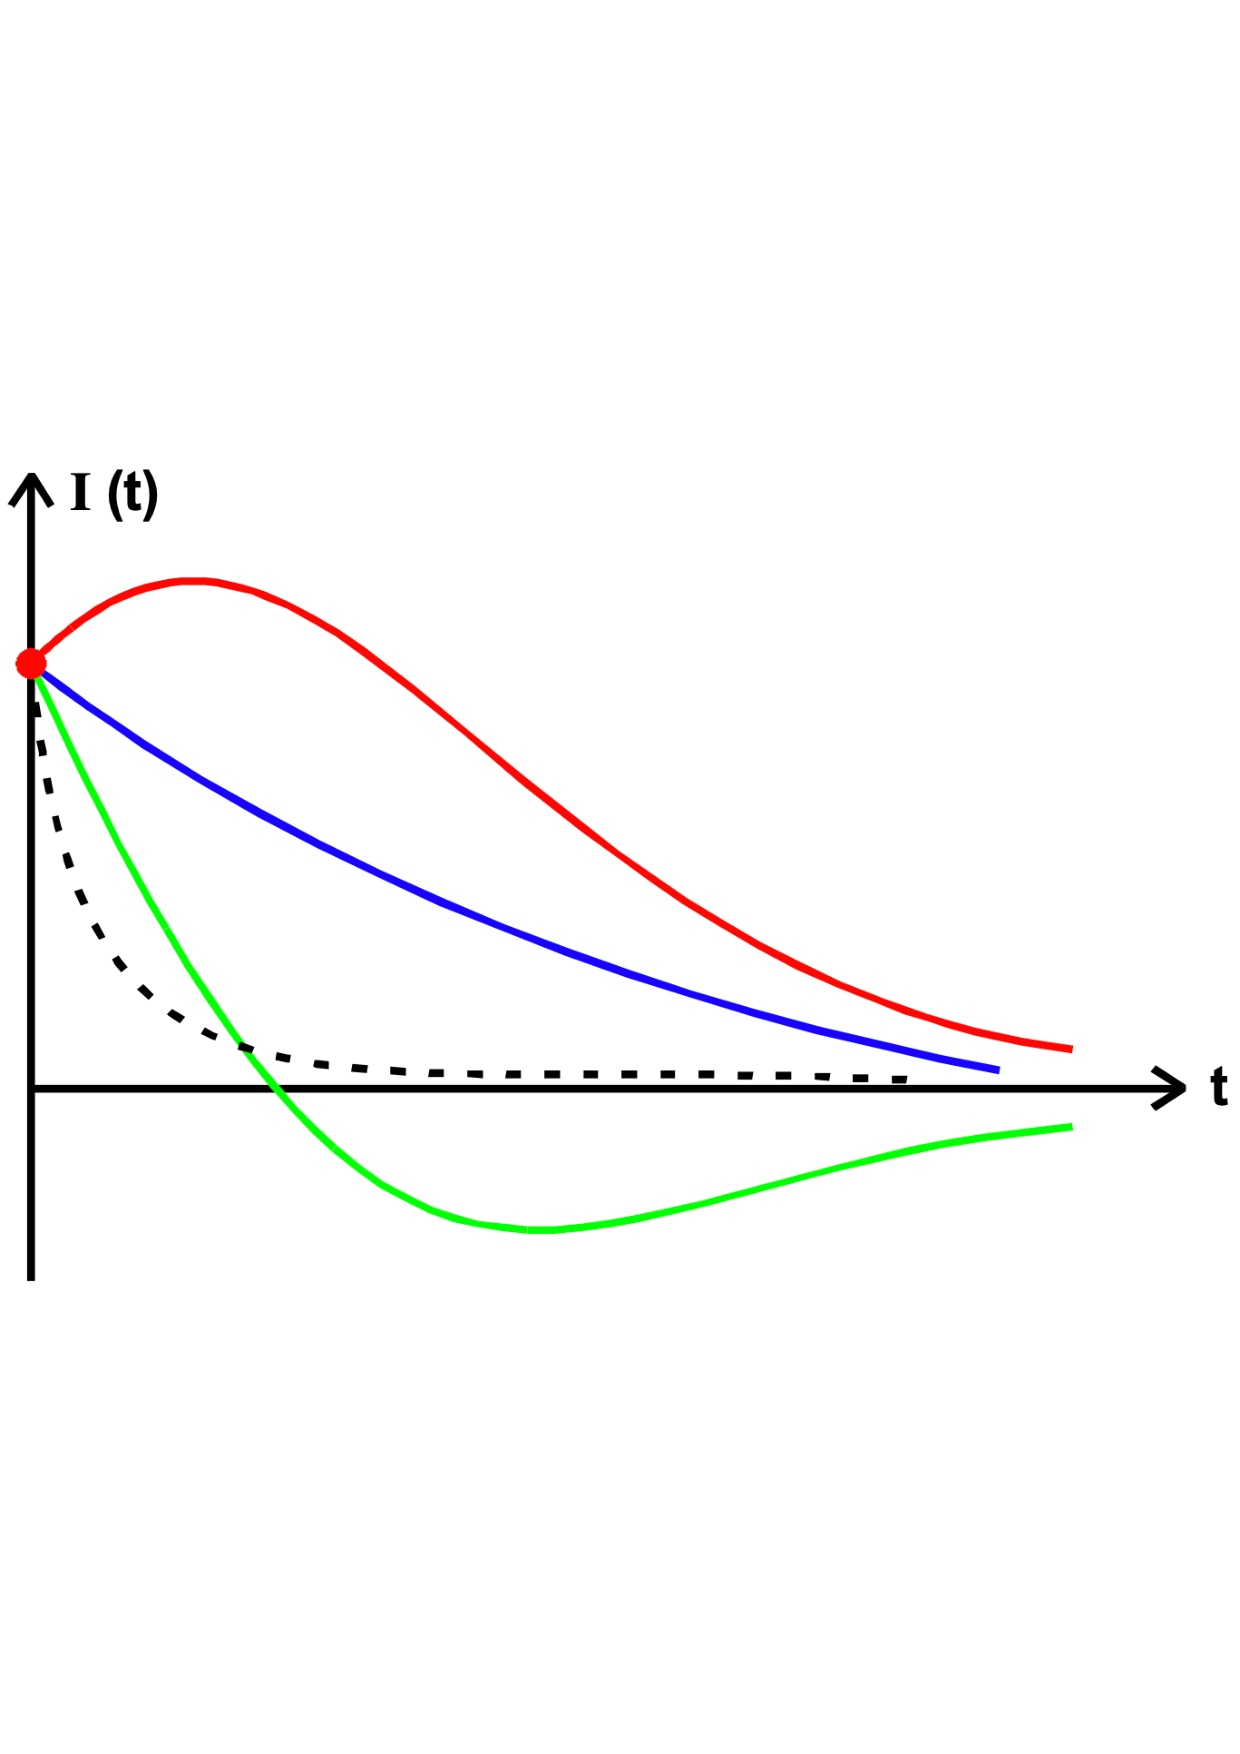
\includegraphics[height=5cm]{grenzfall.pdf}
       \caption{Aperiodischer Grenzfall eines RCL-Kreises (Quelle: \cite{V354}).}
       \label{fig:grenzfall}
\end{figure}

\end{enumerate}

\newpage
\subsection{Erzwungene Schwingung}
Um eine erzwungene Schwingung zu erhalten, wird der Schaltung aus Abbildung (\ref{fig:gedaempft}) ein Generator hinzugefügt,
der eine Wechselspannung liefert, sodass der Aufbau eine wie in Abbildung (\ref{fig:erzwungen}) dargestellte Form hat.

\begin{figure}
    \centering
       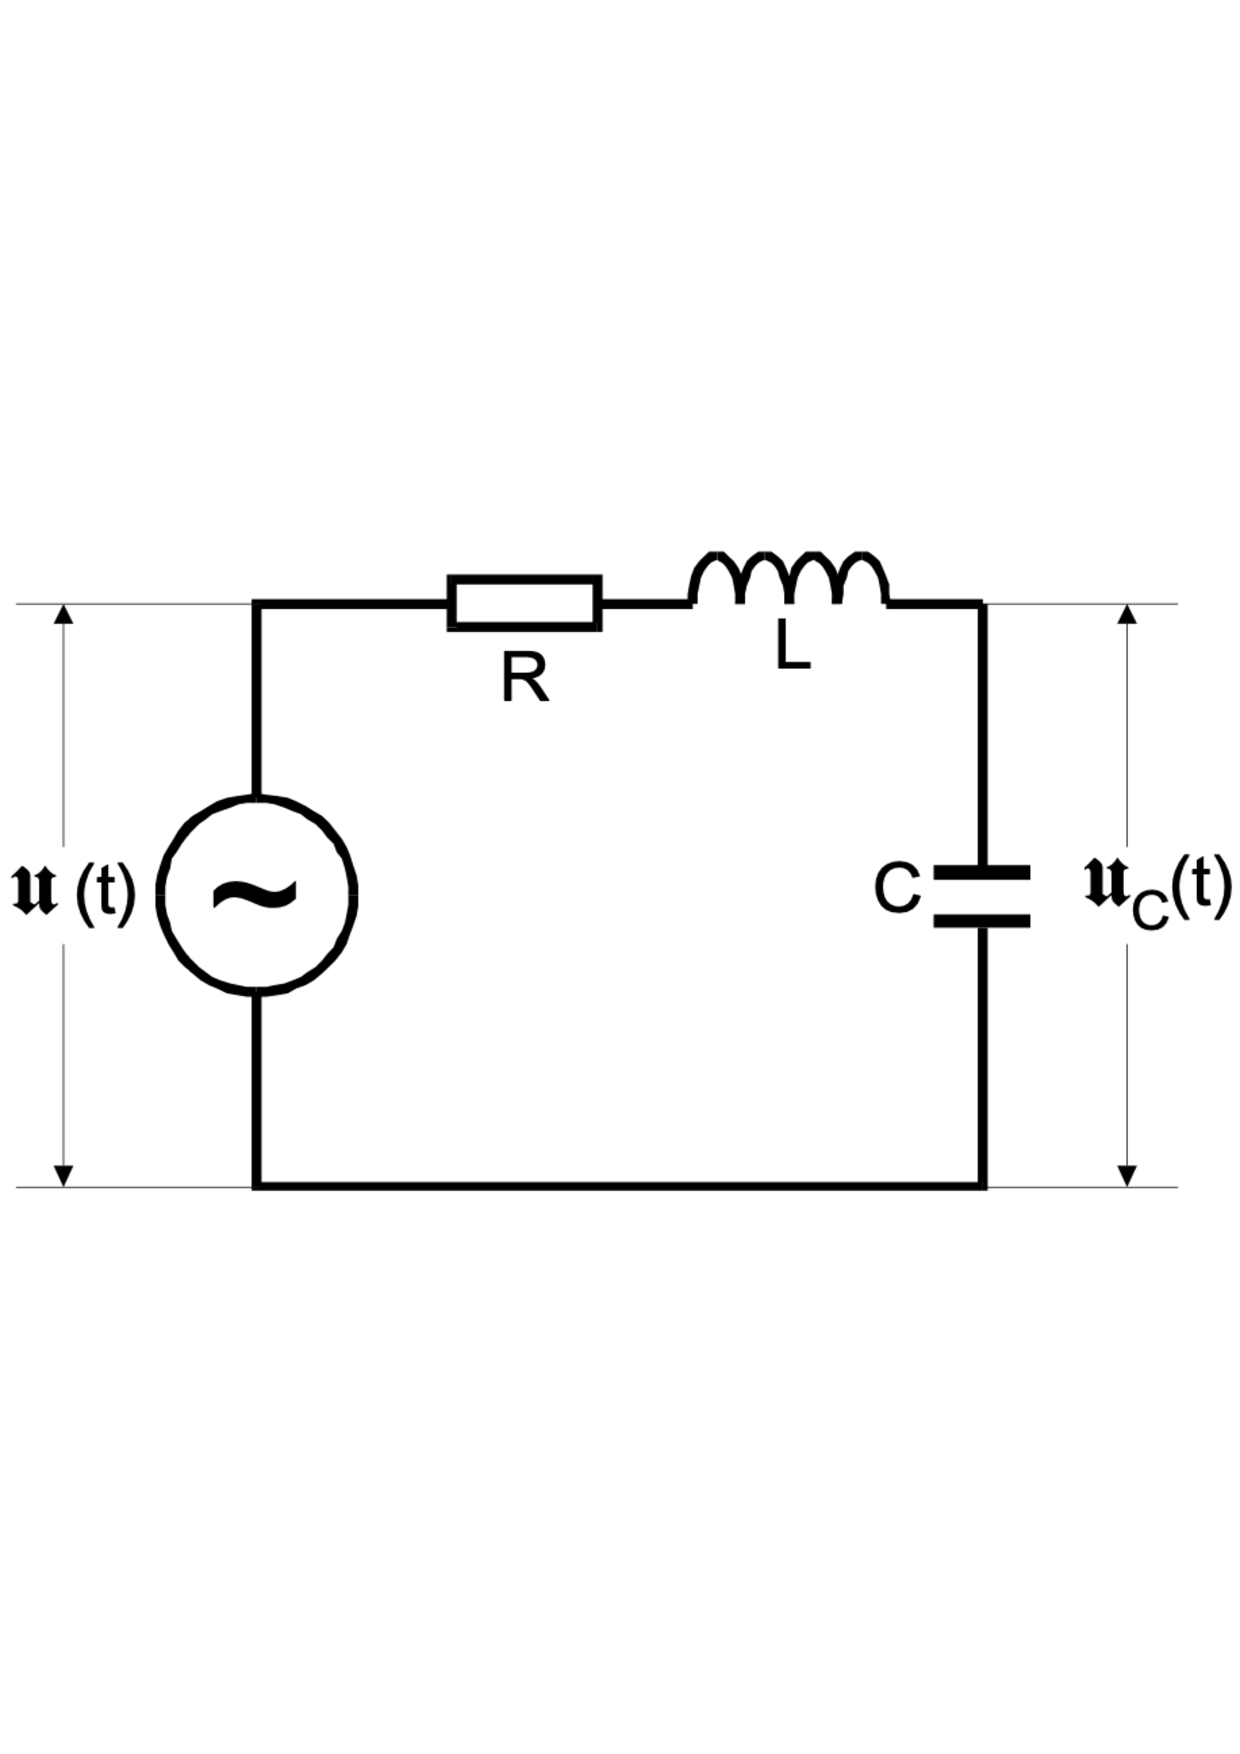
\includegraphics[height=5cm]{erzwungen.pdf}
       \caption{Schaltplan zur Erzeugung einer erzwungenen Schwingung (Quelle: \cite{V354}).}
       \label{fig:erzwungen}
\end{figure}

\noindent
Mit der nun von außen hinzugefügten Energiequelle ergibt sich nach den Kirchhoff'schen Gesetzen eine Differentialgleichung für $U_C$:

\begin{equation}
LC \frac{\text{d}^2 U_C}{\text{dt}^2} + RC \frac{\text{d} U_C}{\text{dt}} + U_C = U_0 e^{j \omega t}.
\end{equation}

\noindent
Mit geeignetem Ansatz kann aus dieser Differentialgleichung eine Funktion für $U_C(\omega)$ ermittelt werden:

\begin{equation}
U_C(\omega) = \frac{U_0}{\sqrt{(1-LC\omega^2)^2 + \omega^2 R^2 C^2}}.
\label{eqn:uc}
\end{equation}

\noindent
Dabei gibt es eine Resonanzfrequenz $\omega_{res}$, bei der $U_C(\omega)$ einen höheren Wert als $U_0$ annehmen kann.
Sie ist definiert als:

\begin{equation}
\omega_{res} = \sqrt{\frac{1}{LC} - \frac{R^2}{2L^2}}.
\label{eqn:res}
\end{equation}

\noindent
Für eine schwache Dämpfung mit $\frac{R^2}{2L^2} << \frac{1}{LC}$ ergibt sich für die Resonanzfrequenz (\ref{eqn:res}) die Kreisfrequenz $\omega_0$ der ungedämpften Schwingung.
In diesem Fall übertrifft $U_C$ die Erregerspannung $U_0$ um den Faktor $\frac{1}{\omega_0 RC}$, 
der als Resonanzüberhöhung oder Güte q des Schwingkreises bezeichnet wird.

\noindent
Die Güte q hängt dabei mit der Breite der Resonanzkurve zusammen, 
die durch die Frequenzen $\omega_+$ und $\omega_-$ charakterisiert sind,
bei denen $U_C$ auf den Bruchteil $\frac{1}{\sqrt{2}}$ seines Maximalwertes abgesunken ist.
Der Zusammenhang kann geschrieben werden als:

\begin{equation}
q = \frac{\omega_0}{\omega_- - \omega_+}= \frac{1}{\sqrt{LC}(\omega_- - \omega_+)}.
\label{eqn:guete}
\end{equation}

\noindent
mit

\begin{equation}
    \omega_- - \omega_+ \approx \frac{R}{L}
    \label{eqn:wmp}
\end{equation}
 


